\documentclass[a4paper,12pt]{article}
\usepackage[a4paper, top=2cm,bottom=2cm,right=2cm,left=2cm]{geometry}

\usepackage{bm,xcolor,mathdots,latexsym,amsfonts,amsthm,amsmath,
					mathrsfs,graphicx,cancel,tikz-cd,hyperref,booktabs,caption,amssymb,amssymb,wasysym}
\hypersetup{colorlinks=true,linkcolor=blue}
\usepackage[italian]{babel}
\usepackage[T1]{fontenc}
\usepackage[utf8]{inputenc}
\newcommand{\s}[1]{\left\{ #1 \right\}}
\newcommand{\sbarra}{\backslash} %% \ 
\newcommand{\ds}{\displaystyle} 
\newcommand{\alla}{^}  
\newcommand{\implica}{\Rightarrow}
\newcommand{\iimplica}{\Leftarrow}
\newcommand{\ses}{\Leftrightarrow} %se e solo se
\newcommand{\tc}{\quad \text{ t. c .} \quad } % tale che 
\newcommand{\spazio}{\vspace{0.5 cm}}
\newcommand{\bbianco}{\textcolor{white}{,}}
\newcommand{\bianco}{\textcolor{white}{,} \\}% per andare a capo dopo 																					definizioni teoremi ...


% campi 
\newcommand{\N}{\mathbb{N}} 
\newcommand{\R}{\mathbb{R}}
\newcommand{\Q}{\mathbb{Q}}
\newcommand{\Z}{\mathbb{Z}}
\newcommand{\K}{\mathbb{K}} 
\newcommand{\C}{\mathbb{C}}
\newcommand{\F}{\mathbb{F}}
\newcommand{\p}{\mathbb{P}}

%GEOMETRIA
\newcommand{\B}{\mathfrak{B}} %Base B
\newcommand{\D}{\mathfrak{D}}%Base D
\newcommand{\RR}{\mathfrak{R}}%Base R 
\newcommand{\Can}{\mathfrak{C}}%Base canonica
\newcommand{\Rif}{\mathfrak{R}}%Riferimento affine
\newcommand{\AB}{M_\D ^\B }% matrice applicazione rispetto alla base B e D 
\newcommand{\vett}{\overrightarrow}
\newcommand{\sd}{\sim_{SD}}%relazione sx dx
\newcommand{\nvett}{v_1, \, \dots , \, v_n} % v1 ... vn
\newcommand{\ncomb}{a_1 v_1 + \dots + a_n v_n} %a1 v1 + ... +an vn
\newcommand{\nrif}{P_1, \cdots , P_n} 
\newcommand{\bidu}{\left( V^\star \right)^\star}

\newcommand{\udis}{\amalg}
\newcommand{\ric}{\mathfrak{U}}
\newcommand{\inclu}{\hookrightarrow }
%ALGEBRA

\newcommand{\semidir}{\rtimes}%semidiretto
\newcommand{\W}{\Omega}
\newcommand{\norma}{\vert \vert }
\newcommand{\bignormal}{\left\vert \left\vert}
\newcommand{\bignormar}{\right\vert \right\vert}
\newcommand{\normale}{\triangleleft}
\newcommand{\nnorma}{\vert \vert \, \cdot \, \vert \vert}
\newcommand{\dt}{\, \mathrm{d}t}
\newcommand{\dz}{\, \mathrm{d}z}
\newcommand{\dx}{\, \mathrm{d}x}
\newcommand{\dy}{\, \mathrm{d}y}
\newcommand{\amma}{\gamma}
\newcommand{\inv}[1]{#1^{-1}}
\newcommand{\az}{\centerdot}
\newcommand{\ammasol}[1]{\tilde{\gamma}_{\tilde{#1}}}
\newcommand{\pror}[1]{\mathbb{P}^#1 (\R)}
\newcommand{\proc}[1]{\mathbb{P}^#1(\C)}
\newcommand{\sol}[2]{\widetilde{#1}_{\widetilde{#2}}}
\newcommand{\bsol}[3]{\left(\widetilde{#1}\right)_{\widetilde{#2}_{#3}}}
\newcommand{\norm}[1]{\left\vert\left\vert #1 \right\vert \right\vert}
\newcommand{\abs}[1]{\left\vert #1 \right\vert }
\newcommand{\ris}[2]{#1_{\vert #2}}
\newcommand{\vp}{\varphi}
\newcommand{\vt}{\vartheta}
\newcommand{\wt}[1]{\widetilde{#1}}
\newcommand{\pr}[2]{\frac{\partial \, #1}{\partial\, #2}}%derivata parziale
%per creare teoremi, dimostrazioni ... 
\theoremstyle{plain}
\newtheorem{thm}{Teorema}[section] 
\newtheorem{ese}[thm]{Esempio} 
\newtheorem{ex}[thm]{Esercizio} 
\newtheorem{fatti}[thm]{Fatti}
\newtheorem{fatto}[thm]{Fatto}

\newtheorem{cor}[thm]{Corollario} 
\newtheorem{lem}[thm]{Lemma} 
\newtheorem{al}[thm]{Algoritmo}
\newtheorem{prop}[thm]{Proposizione} 
\theoremstyle{definition} 
\newtheorem{defn}{Definizione}[section] 
\newcommand{\intt}[2]{int_{#1}^{#2}}
\theoremstyle{remark} 
\newtheorem{oss}{Osservazione} 
\newcommand{\di }{\, \mathrm{d}}
\newcommand{\tonde}[1]{\left( #1 \right)}
\newcommand{\quadre}[1]{\left[ #1 \right]}
\newcommand{\w}{\omega}

% diagrammi commutativi tikzcd
% per leggere la documentazione texdoc

\begin{document}
\textbf{Lezione del 1 aprile}
\begin{thm}Sia $D\subseteq \C$ un aperto e $\w$ una 1-forma su $D$.\\
I seguenti fatti sono equivalenti
\begin{enumerate}
\item $\w$ \`e chiusa
\item $\int_{\partial R} \w=0$ per ogni rettangolo $R\subset D$
\item $\int_\amma \w =0$ per ogni laccio $\amma$ omotopo al laccio costante
\end{enumerate}
\proof  1 $\implica 2$ Se $\amma\sim c$ a estremi fissi dove $c$ \`e il cammino costante allora
$\int_\amma \w =\int_c\w =0$.\\
3 $\implica $ 2. $\partial R$ \`e un cammino omotopicamente banale.\\
2 $\implica$ 1 Visto nella lezione precedente
\end{thm}

Ricordiamo che ogni cammino chiuso $\amma:\, [0,1]\to D$ definisce un loop $\hat{\amma}:\, S^1 \to D$
\begin{defn}[Liberamente omotopo]\bianco
Siano $\alpha, \gamma$ loop.\\
$\gamma$ si dice liberamente omotopo a $\alpha$ se
$$\exists H:\, [0,1]\times [0,1]\to [0,1] \to D$$ 
continua con 
$$H(t,0)=\gamma(t) $$
$$H(t,1)=\alpha(t)$$
$$H(0,s)=H(1,s) \, \forall s $$
\end{defn}
\begin{oss}Due cammini sono liberamente omotopi se esiste un omotopia tra loro $H$ tale che 
$$H(\bullet, s):\, [0,1]\to D$$ 
\`e un cammino chiuso per ogni $s$.\\
Tale condizione \`e una condizione pi\`u debbole dell'omotopia ad estremi fissi in quanto $H(0,s) = H(1,s)$ non sono costanti in $s$
\end{oss}

\begin{prop}
$$ \alpha \text{ liberamente omotopo a } \gamma \quad \ses \quad \hat{\alpha}\sim \hat{\gamma} \quad \ses\quad \exists\beta \text{ cammino } \gamma \sim \beta \star \alpha \star \overline{\beta} \text{ ad estremi fissi } $$
\end{prop}
\begin{ese}in $\C\setminus\s 0 $ i cammini $\gamma(t) =e^{2\pi i t} $ e $\alpha(t) = 5e^{2\pi it}$ sono liberamente omotopi 
\end{ese}
\begin{fatto}Se $\w$ \`e una $1$-forma chiusa su $D$ e $\alpha, \gamma$ sono cammini chiusi liberamente omotopi allora
$$ \int_\amma \w = \int_\alpha \w$$
infatti $\gamma \sim \beta \star \alpha\star \overline{\beta}$ ad estremi fissi dunque 
$$ \int_\gamma \w = \int_{\beta \star \alpha\star \overline{\beta}} \w = \int_\beta \w +\int_\alpha \w = \int_{\overline{\beta}} \w = \int_\alpha\w$$
\end{fatto}
\newpage
\section{Forme chiuse di classe $C^1$}
\begin{defn}Sia $D\subseteq \C$ 
aperto e $\w=P \dx + Q\dy $ $1$-forma su $D$.\\
$\w$ si dice $C^1$ se $P,Q:\, D\to \C$ sono funzioni di classe $C^1$.\\
In questo caso poniamo formalmente
$$ \di \w = \tonde{\pr Q x- \pr P y }\dx \dy$$
(la definizione \`e formale in quanto non diamo significato a $\dx\dy$ \`e un simbolo formale)
\end{defn}
\spazio
Andiamo ora a definire l'integrazione su un rettangolo.\\
Sia $R\subset \C$ un rettangolo e $f:\, R \to \C$ continua, allora ha senso $\int_R f(x,y) \dx\dy$.\\
Se $(a_1,b_1), \, (a_2, b_1),\, (a_2, b_2), \, (a_1,b_2)$ sono i vertici del rettangolo allora 
$$ \int_R f(x,y)\dx\dy = \int_{[a_1,a_2]\times [b_1, b_2]} f(x,y) \dx \dy = \int_{a_1}^{a_2}\left( \int_{b_1}^{b_2} f(x,y) \dy \right) \dx = 
\int_{b_1}^{b_2}\left( \int_{a_1}^{a_2} f(x,y) \dx \right) \dy$$
\begin{thm}[Formula di Green, Green-Rieman, Stokes]
Sia $\w$ una $1$-forma $C^1$ du $D$ e $R\subseteq D$ un rettangolo allora
$$ \int_{\partial R } \w = \int_R \di w$$
\proof Con le notazioni appena introdotte
$$ \int_R \di w = \int_R \tonde{\pr Q x - \pr P y }\dx\dy = \int_R \pr Q x \dx \dy - \int_R \pr P y \dx \dy = $$
$$=\int_{b_1}^{b_2} \tonde{ \int_{a_1}^{a_2} \pr Q x \dx} \dy - \int_{a_1}^{a_2} \tonde{ \int_{b_1}^{b_2} \pr P y \dy} \dx =$$
$$ \int_{b_1}^{b_2} \tonde{ Q(a_2, y) -Q(a_1,y)} \dy - \int_{a_1}^{a_2} \tonde{ P(x,b_2) - P(x,b_1)} \dx =$$
$$ \int_{b_1}^{b_2} Q(a_2,y)\dy -\intt{b_1}{b_2} Q(a_1,y) \dy - \intt{a_1}{a_2} P(x,b_2) \dx + \intt{a_1}{a_2} P(x,b_1) \dx = \int_{\partial R } \w$$
\endproof 
\end{thm}
\spazio
\begin{thm}Sia $\w$ una $1$-forma $C^1$ su $D$ 
$$ \w \text{ chiusa } \quad \ses \quad \di \w =0$$
\proof $\implica $ Essendo la forma chiusa, $\forall p\in D$ esiste $U\subseteq D$ aperto con $p\in U$ e con
$$ \w = \pr F x \dx + \pr F y \dy \text{ su } U$$
Essendo $\w$ di classe $C^1$, $F$ \`e di classe $C^2$ ora
$$ \di \w = \left( \frac{\partial}{\partial x}\left( \pr F y \right) -  \frac{\partial}{\partial y}\left( \pr F x \right) \right) \dx \dy $$
ora per un noto teorema
$$ \frac{\partial^2 F}{\partial x \partial y } = \frac{\partial^2 F}{\partial y \partial x }$$
da cui $\di \w=0$\\
$\iimplica$ Sia $R\subset D$ un  rettangolo. Allora  per il teorema precedente
$$ \int_{\partial R}\w =\int_R \di \w =0$$
dunque per un teorema precedente $\w$ \`e chiusa 
\endproof
\end{thm}
\newpage
\begin{thm}Sia $f:\, D \to \C$ olomorfa. $f(z)\di z $ \`e una $1$-forma chiusa su $D$ 
\proof Supponiamo $f(z) \di z $ non sia chiusa, allora esiste un rettangolo $R\subseteq D$ tale che $\int_{\partial R} \w \neq 0$.\\
D'ora in avanti se $\overline{R}$ \`e un rettangolo denoteremo $\alpha(\overline{R})=\int_{\partial \overline{R}} \w$.\\
Dividiamo il rettangolo $R$ in $4$ rettangoli congruenti (dividiamo a met\`a entrambi i lati) ottenendo cos\`i i rettangoli $A_1, \dots, A_4$, osserviamo 
$$ \alpha(R) =\alpha(A_1) +\dots + \alpha(A_4)$$
in quanto nel membro a destra, i contributi dei segmenti interni si elidono.\\
Essendo $\alpha(R)\neq 0$ esiste un $A_i$ tale che 
$$ \abs{\alpha(A_i)}\geq \frac{\abs{\alpha(R)}}{4}$$ 
Pongo $R_1$ uguale ad $A_i$, iterando la costruzione applicandola ad $R_1$ ottengo un nuovo rettangolo $R_2\subset R_1$ tale che $\abs{\alpha(R_2)}\geq \frac{\abs{\alpha(R_1)}}{2}\geq \frac{\abs{\alpha(R_1)}}{4}$.\\
Iterando tale costruzione ottengo una successione di rettangoli inscatolati $$R_1 \supset R_2 \supset \cdots \supset R_n \supset\cdots$$
con 
$$ \abs{\alpha(R_i)}> \frac{\abs{\alpha(R)}}{4^i}$$
Sia $z_0\in \bigcap_{n\in \N} R_n\neq \emptyset$ (essendo intersezione di compatti chiusi non vuoti).\\
Poich\`e $f$ olomorfa 
$$ f(z) = f(z_0) + f'(z_0) (z-z_0) + \varepsilon (z) \abs{z-z_0}$$
dove 
$$ \lim_{z\to z_0} \abs{\varepsilon(z)} \to 0 $$ 
dunque 
$$ \alpha(R_n) =\int_{\partial R_n} \left( f(z_0) +f'(z_0) (z-z_0) +\varepsilon(z) \abs{z-z_0} \right) \di z =$$
$$\int_{\partial R_n} f(z_0)\di z   + \int_{\partial R_n} f'(z_0) (z-z_0) \di z +\int_{\partial R_n} \varepsilon(r) \abs{z-z_0} \di z 
= \int_{\partial R_n} \varepsilon(r) \abs{z-z_0} \di z $$
infatti $\di z $ e $(z-z_0)\di z $ sono esatte ammettendo come primitiva $z$ e $\frac{(z-z_0)^2}{2}$.\\
Se $n$ \`e sufficientemente grande, $R_n\subseteq B(z_0, \delta)$ con $\delta$ piccolo a piacere.\\
Inoltre possiamo scegliere $n$ in modo che 
$$ \abs{\varepsilon(z) } \leq \frac{\abs{\alpha(R)}}{4(a+b)^2} \quad \forall z\in R_n$$
dove $a,b$ sono le lunghezze dei lati di $R$. Tale scelta \`e possibile in quanto $diam(R_n) \leq \frac{a+b}{2^n}$ e $\varepsilon(z) \to 0 $ per $z\to z_0$.\\
Per tale $n$ se $z\in \partial R_n$  si ha $\abs{z-z_0} \leq \frac{a+b}{2^n}=diam(R_n)$ per cui 
$$ \abs{\alpha(R_n)} = \abs{\int_{\partial R_n } \varepsilon(z) \abs{z-z_0} \di z } \leq 
$$$$\leq \int_{0}^{2\frac{a+b}{2^n}} 
\abs{\varepsilon(\gamma(t))} \cdot \abs{\gamma(t) - z_0} \dt \leq \frac{2(a+b)}{2^n} \cdot \frac{\abs{\alpha(R)}}{4(a+b)^2}\cdot \frac{a+b}{2^n} =\frac{1}{2}\cdot \frac{\abs{\alpha(R)}}{4^n}$$
il che contraddice $\abs{\alpha(R_n)} > \frac{\abs{\alpha(R)}}{4^n}$\\
$\gamma $\`e un cammino che parametrizza il bordo di $R_n$
\endproof
\end{thm}

\begin{cor}Sia $f:\, D\to \C$ olomorfa allora $\forall p\in D$ esiste $U\subseteq D$ aperto con $p\in U $ e $F:\, U \to C$ olomorfa con $F'=f_{\vert U} $
\proof $f(z) \di z $ \`e chiusa, dunque esiste $U$ come nell'enunciato e $F:\, U \to \C$ con $\di F=f(z) \di z $ su $U$.\\
Abbiamo $F$ olomorfa e $F'=f$ su $U$ 
\endproof
\end{cor}
\begin{cor}Sia $f:\, D \to \C$ olomorfa, allora $\int_\gamma f(z) \di z =0$ per ogni laccio $\gamma$ omotopicamente banale
\end{cor}
\spazio
\begin{prop}Sia $f:\, D \to \C$ con $D\subseteq  \C$ aperto.\\
Se $f$ \`e continua su $D$ e olomorfa su $D\setminus r $ dove $r$ retta orizzontale, allora $f(z) \di z $ \`e chiusa
\proof Sia $R\subseteq D$ un rettangolo, dimostriamo che $\int_{\partial R} f(z)\di z=0$.\\
Andiamo a distinguere alcuni  casi 
\begin{itemize}
\item Se $r\cap R=\emptyset$ allora $f$ olomorfa su tutto $R$ dunque ricadiamo nel teorema precedente
\item Se un lato orizzontale di $R$ giace su $r$ allora costruisco una successione di rettangoli $R_n$ come in figura 
\begin{figure}[!h]
\centering 
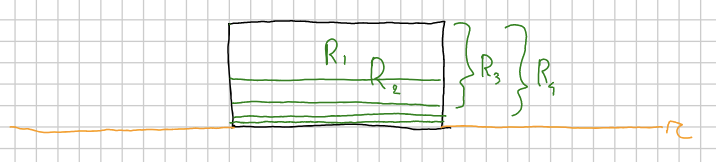
\includegraphics{Figure/04_01}
\end{figure}
in modo che $R_n$ "tenda" a $R$.\\
Allora usando che $f$ \`e continua si vede
$$ \int_{\partial R} f(z) \di z = \lim_{n\to +\infty} f(z) \di z  =0$$ 
in quanto $\int_{\partial R_n} f(z) \di z =0$ per ogni $n$ ($r$ non initerseca la retta e ricadiamo nel caso precedente).\\
Se $R$ ha vertici $(a_1, b_1), \, (a_2,b_1), \, (a_2,b_2), \, (a_1,b_2)$ e $R\cap r$ ha ordinata $b_1$ con $b_1<b_2$ allora i vertici di $R_n$ sono $\tonde{a_1, b_1+\frac{1}{n}},\, \tonde{a_2, b_1+\frac{1}{n}},\, \tonde{a_2,b_2} , \,  (a_1,b_2)$
\item Se $r$ interseca $R$ ma $r$ non contiene lati di $R$, allora $r$ divide il rettangolo in $2$ rettangoli $R_1$ e $R_2$.\\
Ora un lato di $R_1$ giace su $r$, cos\`i come per $R_2$ concludiamo osservando che 
$$ \int_{\partial R} f(z) \di z = \int_{\partial R_1} f(z) \di z + \int_{\partial R_2} f(z)\di x = 0+0 = 0 $$
\end{itemize}
\end{prop}
\end{document}